\clearpage
\section{Zmiany wdrożeniowe projektu GGSS}
\label{ch:scripts}


Niniejsza część pracy opisuje zmiany związane ze skryptami służącymi do obsługi projektu GGSS w środowisku docelowym. Opisowi poddane zostały wprowadzone w nich zmiany, nowe funkcjonalności, czy też usprawnienia mające na celu poszerzenie możliwości wdrożeniowe projektu GGSS. Przedstawione zostały również rozwinięcia wdrożeniowe w automatyzacji projektu GGSS.

\subsection{Wprowadzenie do problematyki}

W celu zapewnienia obsługi systemu ggss w środowisku produkcyjnym oraz łatwości korzystania istniało wiele skryptów, które pozwalały na wdrożenie aplikacji. Odpowiadały one między innymi za obsługę cyklu życia aplikacji, np.: poprzez komendy \lstinline{start}, \lstinline{stop}, \lstinline{remove_lock}, \lstinline{check} wsparane przez skrypt \lstinline{ggss_monitor}. Co więcej skrypty te w połączeniu z aplikacją \lstinline{crontab}, odpowiedzialną za cykliczne wykonywanie komend na systemach z rodziny Linux, zapewniały ciągłe działanie aplikacji GGSS oraz uruchamianie jej z odpowiednimi prawami dostępu. Oprócz skryptów wdrożeniowych w ramach systemu GGSS istniała również infrastruktura odpowiedzialna za awaryjne wyłączenie zasilania na zasilaczu wysokiego napięcia.

\subsection{Motywacja do wprowadzenia zmian}
\label{sec:scripts_motiv}

Ze względu na sposób implementacji poprzednich skryptów w celu poprawnego działania wymagane było, aby w systemie docelowym istniała określona struktura katalogów, a wewnątrz niej znajdowały się aplikacje projektu GGSS. Dodatkowo logika potrzebna do działania systemu rozbita była na wiele plików-skryptów luźno ze sobą powiązanych, z niewiele tłumaczącymi nazwami. W celu dowiedzenia się co dany skrypt robi trzeba było sprawdzać jego zawartość, bądź być dobrze zaznajomionym ze skrótami użytymi w nazwie. Ze względu na powyższe czynniki postanowiono usprawnić skrypty odpowiadające za obsługę projektu ggss w systemie docelowym. Dodatkowo postanowiono rozszerzyć możliwości skryptów o monitorowanie zasobów zużywanych przez główną aplikację projektu GGSS.

Modyfikacji została poddana również infrastruktura odpowiedzialna za awaryjne wyłączanie zasilania. Po analizie jej obecnych możliwości oraz uzyskaniu wymagań co do infrastruktury okazało się, że nie spełnia ona założeń. Najważniejszym przypadkiem użycia dla tejże infrastruktury było wyłączenie zasilania w momencie, gdy główna aplikacja projektu GGSS przestaje działać. Oprócz tego zabezpieczeniu miał zostać poddany proces wyłączania maszyny (ang. \emph{shutdown}), tak, aby po zamknięciu systemu operacyjnego na komputerze produkcyjnym kanały wszystkich zasilaczy zostały wyłączone. Infrastruktura w pierwotnej postaci wspierała jedynie ten drugi przypadek.

Ze względu na brak ustandaryzowanego oraz łatwego sposobu na pozyskanie aplikacji, pakietów oraz skryptów potrzebnych na wdrożenie systemu ggss w środowisko docelowe postanowiono wzbogacić automatyzację o kroki konsolidujące wszystkie zasoby potrzebne do wdrożenia projektu w środowisko produkcyjne wraz z ich odpowiednim opisaniem.

\subsection{Skrypt do monitorowania zużytych zasobów przez główną aplikację ggss}

W ramach pracy inżynierskiej został przygotowany skrypt \lstinline{check_mem_ggssrunner.sh}, którego zadaniem było sprawdzanie zużycia pamięci, a dokładniej parametru VSZ (\emph{Virtual Memory Size}), który reprezentował ilość pamięci do której na dany moment miał dostęp proces, między innymi: pamięc na partycji wymiany (ang. \emph{swap}), pamięc zaalokowana (również ta nieużywana), pamięć przeznaczona na biblioteki współdzielone. Ze względu na to, że parametr ten nie oddawał dobrze zużywanej pamięci przez aplikację postanowiono rozbudować wyżej wymieniony skrypt o następujące parametry:
\begin{itemize}
    \item CPU - stosunek wykorzystanego czasu procesora do rzeczywistego czasu, który upłynął od uruchomienia procesu
    \item MEM - stosunek RSS do całkowitej fizycznej pamięci zainstalowanej w systemie
    \item RSS (\emph{Resident Set Size}) - ilość pamięci RAM wykorzystywanej przez proces. Brane pod uwagę są również biblioteki współdzielone załadowane do pamięci, wykorzystywane przez proces. Nie zawiera informacji o pamięci na partycji wymiany. \cite{rssvsz}
\end{itemize}
RSS dokładniej ukazuje pamięc wykorzystywaną przez proces. W przypadku monitorowania z użyciem jedynie VSZ możemy łatwo pominąć niepokojące zachowanie aplikacji, ponieważ w zaalokowanej pamięci nie będzie to widoczne.

Skrypt został rozbudowany również o system, który pozwala na nieprzerwane działanie w tle bez błędów nawet, gdy główna aplikacja ggss pozostaje nieuruchomiona. Wyświetlany jest wówczas stosowny komunikat zamiast standardowych statystyk. Efekt ten uzyskano dzięki wykorzystaniu szeregu połączonych ze sobą, za pomocą tak zwanych \emph{pipe}, programów środowiska Linux, tj.: \emph{grep, ps} \cite{man} oraz \emph{awk}. Odpowiednie połączenie tych komend pozwala na uzyskanie identyfikatora procesu (PID - \emph{Process Identifier}) i zapisanie go w zmiennej. W przypadku, gdy aplikacja nie jest uruchomiona zmienna pozostanie pusta. Wykorzystując język Bash, jego struktury warunkowe oraz wyżej wymienioną zmienną możliwe było utworzenie zachowania zależnego od tego, czy proces jest uruchomiony, czy też nie.

\subsection{Zmiany w skryptach operacyjnych}

Przed dokonaniem zmian w skryptach operacyjnych, w pierwszej kolejności dokonano analizy wykorzystywanych skryptów i usunięto te, które nie były już potrzebne. Były to skrypty: \lstinline{dimhw_mon_vmon.sh}, \lstinline{dimhw_det_all_off.sh} oraz \lstinline{ggss_starter.sh}. Pierwsze dwa z nich nie mogłyby zostać wykorzystane po wprowadzonych zmianach w systemie, ponieważ modyfikacji uległ format komend obsługiwanych przez projekt GGSS, które mają kontrolować działanie zasilacza wysokiego napięcia. Natomiast ostatni z nich został usunięty, ponieważ logika zawarta w ramach tego skryptu została przeniesiona do pliku \lstinline{ggss_monitor.sh}, czyli jedynego miejsca, gdzie była ona wykorzystywana.

Jedną z ważniejszych zmian było wprowadzenie zmian w skryptach, które możliwiły umieszczanie projektu ggss w dowolnej ścieżce w systemie. W początkowej wersji skryptów operacyjnych zapisana była na stałe ścieżka \lstinline{/localdisk/ggss/bin}. Obecnie ścieżka jest odczytywana względem umiejscowienia skryptów. Ze względu na to, że skrypty te cyklicznie uruchamiane są przez aplikację \lstinline{crontab} niemożliwe było skrozystanie ze ścieżki względnej (\lstinline{./}) konieczne za to było wykorzystanie parametru \lstinline{BASH_SOURCE}, który jest tablicą, a element o indeksie 0 zawiera informację o względnej ścieżce, gdzie znajduje się wywoływany skrypt. Aby otrzymać ścieżkę bezwzględną wykorzystane zostało połączenie wyżej opisanego parametru waraz z komendą \lstinline{cd} oraz \lstinline{pwd}. Zamieniając wszystkie wystąpienia \lstinline{/localdisk/ggss/bin} na uzyskaną we wcześniej opisany sposób ścieżkę bezwzględną efektywnie pozwoliło na umieszczanie projektu ggss w dowolnej ścieżce w systemie.

W skryptach operacyjnych dokonano również małego usprawnienia w systemie sprawdzającym, czy główna aplikacja systemu GGSS jest uruchomiona. W pierwotnej wersji system jedynie sprawdzał, czy aplikacja \emph{ggss-runner} jest uruchomiona. Dodatkowo system ten mógł łatwo ulec błędnemu działaniu, ponieważ wyniki nie były poprawnie filtrowane. Działanie polegało na sprawdzeniu, czy po odfiltrowaniu standardowego wyjścia z komendy \lstinline{ps} za pomocą komendy \lstinline{egrep} zawierającej jako argument nazwę aplikacji pozostaje jakakolwiek wartość. Szczęśliwie argument komendy filtrującej poprzedzony był prefiksem \lstinline{./} dzięki czemu system działał poprawnie. Natomiast gdyby prefiks ten nie występował to nawet w przypadku gdyby aplikacja \emph{ggss-runner} nie była uruchomiona odflitrowany wynik działania zawierałby w sobie komendę \lstinline{egrep}, co przedstawia listing \ref{lst:egrep_error}. W celu zapobiegnięcia w przyszłości problemów z systemem weryfikowania, czy główna aplikacja projektu GGSS jest uruchomiona wprowadzono dodatkowy filtr eliminujący z standardowego wyjścia wpisy na temat komendy \lstinline{grep}.

\begin{lstlisting}[language=cmd,caption={Przykładowe działanie połączenie komend ps oraz egrep bez prefixu \lstinline{./} przy argumencie komendy egrep.},label={lst:egrep_error},frame=single]
user@host:~$ ps afux | egrep "ggssrunner"
user  461  0.0  0.0  8160  732 pts/3   S+  14:20  0:00 \_ grep -E --color=auto ggssrunner
\end{lstlisting}

\subsection{Zmiany w systemie awaryjnego wyłączania zasilania}

Ze względu na wymagane zmiany opisane w ramach sekcji \ref{sec:scripts_motiv} oraz chęci autorów do pozbycia się jak największej liczby zewnętrznych zależności w projekcie GGSS wprowadzono szereg zmian w systemie awaryjnego wyłączania zasilania.

Po pierwsze zmianie uległ skrypt \lstinline{wd_hv.sh}, który uruchamiany jest cyklicznie w ramach aplikacji \lstinline{crontab}, a jego celem jest upewnienie się, że skrypt pułapka (ang. \emph{trap}), którego zadaniem jest uruchomienie aplikacji awaryjnego wyłączenia zasilania w przypadku otrzymania sygnały SIGTERM, dla zasilacza wysokiego napięcia jest uruchomiony. Wprowadzone zostały wcześniej opisane zmiany, które pozwoliły na umieszczenie skryptu w dowolnym miejscu w systemie, dodatkowo wprowadzono zmiany usprawniające wykrywanie czy skrypt pułapka jest uruchomiony. Ponadto wprowadzona została funkcjonalność blokowania uruchomienia aplikacji pułapki, nawet, gdy jest ona nieuruchomiona. Zaimplementowane zostało to z użyciem pliku blokady (ang. \emph{lock}). W przypadku występowania pliku \lstinline{high_voltage_killer_trap.lock} w ścieżce, gdzie znajduje się skrypt \lstinline{wd_hv.sh} to skrypt pułapka nie zostanie uruchomiony niezależnie od pozostałych warunków.

W celu zapewnienia awaryjnego wyłączania zasilania na zasilaczu wysokiego napięcia, gdy główna aplikacja projektu ggss pozostaje nieuruchomiona dłużej niż 5 minut, a przed tym okresem czasu była uruchomiona skrypt pułapka został wzbogacony o wykrywanie statusu aplikacji \emph{ggss-runner} oraz o licznik czasu z wykorzystaniem wewnętrznej zmiennej powłoki Bash \emph{SECONDS}. W przypadku, gdy główna aplikacja ggss jest uruchomiona zmienna ta jest zerowana, w przeciwnym wypadku, gdy zmienna ta osiągnie wartość 300, czyli 5 minut, uruchamiana jest aplikacja \emph{high-voltage-killer}, której zadaniem jest wyłączenie napięcia na wyjściu zasilacza.

Aplikacja \emph{high-voltage-killer} została napisana od początku z użyciem języka C++, a jej zasada działania jest identyczna, jak w przypadku pierwotnego rozwiązania w języku Python. W trakcie działania aplikacja łączy się ze wszystkimi dostępnymi zasilaczami podłączonymi w ramach połączenia łańcuchowego, po czym zeruje na nich napięcia. Dodatkowo, ze względu na wykorzystanie języka, który używany jest również w głównej aplikacji systemu GGSS, możliwe było wykorzystanie obsługi zasilacza już istniejącej w ramach biblioteki \emph{caenn1470-lib}. Co więcej stosowanie języka C++ pozwoliło na wyeliminowanie ostatniej zależności w projekcie do biblioteki \emph{python-serial}, a zatem całkowite pozbycie się jej z projektu GGSS.

\subsection{Wdrożenie z użyciem automatyzacji Gitlab CI/CD}

Aby uprościć proces wdrażania systemu GGSS wykorzystano funkcjonalność wydań (ang. \emph{release}) dostępną w ramach portalu GitLab oraz częściowo opisaną w ramach sekcji \ref{ch:versioning}. Przy każdorazowym utworzeniu wydania wszystkie pliki potrzebne do wprowadzenia do systemu docelowego, aby projekt GGSS mógł być uruchomiony, dostępne są z panelu danego wydania co widoczne jest na rysunku \ref{fig:release}. Przygotowana w ten sposób infrastruktura pozwala bez większych problemów na szybkie uzyskianie wszystkich potrzebnych zasobów do uruchomienia projektu ggss, a cały proces jest znacznie uproszczony.

\begin{figure}[H]
    \centering
    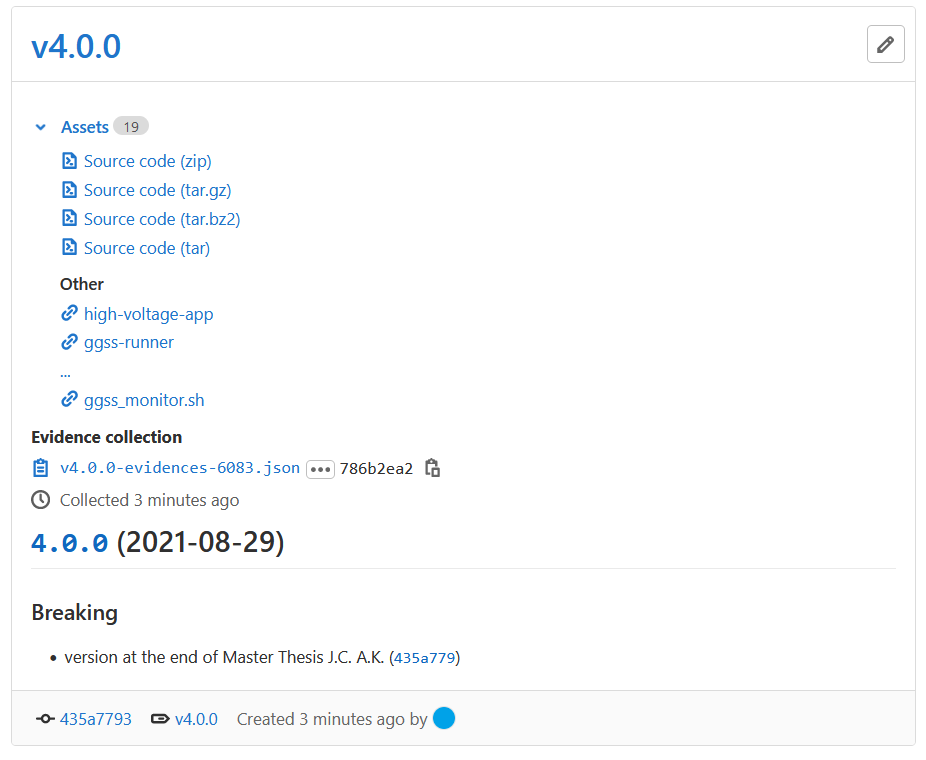
\includegraphics[width=\textwidth]{release.png}
    \caption{Panel wydania projektu GGSS w ramach portalu GitLab.}
    \label{fig:release}
\end{figure}

